% \documentclass[a4paper, conference, compsoc]{IEEEtran}
\documentclass[12pt,a4paper]{article}
\usepackage[bottom=7em]{geometry}
% \documentclass[%
%     pdftex,
%     oneside,			% Einseitiger Druck.
%     12pt,				% Schriftgroesse
%     parskip=half,		% Halbe Zeile Abstand zwischen Absätzen.
% %	topmargin = 10pt,	% Abstand Seitenrand (Std:1in) zu Kopfzeile [laut log: unused]
%     headheight = 12pt,	% Höhe der Kopfzeile
% %	headsep = 30pt,	% Abstand zwischen Kopfzeile und Text Body  [laut log: unused]
%     headsepline,		% Linie nach Kopfzeile.
%     footsepline,		% Linie vor Fusszeile.
%     footheight = 16pt,	% Höhe der Fusszeile
%     abstracton,		% Abstract Überschriften
%     DIV=calc,		% Satzspiegel berechnen
%     BCOR=8mm,		% Bindekorrektur links: 8mm
%     headinclude=false,	% Kopfzeile nicht in den Satzspiegel einbeziehen
%     footinclude=false,	% Fußzeile nicht in den Satzspiegel einbeziehen
%     listof=totoc,		% Abbildungs-/ Tabellenverzeichnis im Inhaltsverzeichnis darstellen
%     toc=bibliography,	% Literaturverzeichnis im Inhaltsverzeichnis darstellen
% ]{scrreprt}	% Koma-Script report-Klasse, fuer laengere Bachelorarbeiten alternativ auch: scrbook


% Basic packages
\usepackage[T1]{fontenc}
\usepackage[utf8]{inputenc}
\usepackage[scaled]{beramono}
\usepackage[english,ngerman]{babel,varioref}
\usepackage{xcolor}
\usepackage{amsmath}

% Tables
\usepackage{booktabs}
\usepackage{multirow}
\usepackage{longtable}
% Graphics and Includes
\usepackage[pdftex]{graphicx}
\graphicspath{{assets/img/}}
\DeclareGraphicsExtensions{.pdf,.jpeg,.png,.jpg}
\usepackage{tikz}
\usetikzlibrary{arrows.meta,bending,automata,shapes}
\usepackage[underline=true,rounded corners=false]{pgf-umlsd}

% Reduce distance before caption
\usepackage[skip=5pt]{caption}
% Bibliography
\usepackage[backend=biber, isbn=false, doi=false, style=ieee]{biblatex}
\addbibresource{bibliography.bib}
\AtBeginBibliography{\raggedright}
%\nocite{*}

% Gossar z.a. für acronyme
% \usepackage[acronym]{glossaries}
% \makeglossaries
\usepackage[printonlyused]{acronym} % falls gewünscht kann die Option footnote eingefügt werden, dann wird die Erklärung nicht inline sondern in einer Fußnote dargestellt

% \section*{Abkürzungsverzeichnis}
\begin{acronym}
    \acro{ps4}[PS4]{Playstation 4}
    \acro{cli}[CLI]{Command Line Interface}
\end{acronym}
% Colors
\definecolor{ListingBackground}{HTML}{FFFFFF}
\definecolor{LinkColor}{HTML}{00007A}


% Font
\usepackage[onehalfspacing]{setspace}
\usepackage{lmodern}
\usepackage[official]{eurosym}
\usepackage{enumitem}
\usepackage[locale=DE]{siunitx} % SI Units für Währungen
\DeclareSIUnit{\EUR}{\text{\euro}} % Beispielverwendung: \SI{10.10}{\EUR}

\usepackage[autostyle=true,german=quotes]{csquotes}
\usepackage{url}
\newcommand{\code}[1]{\texttt{#1}}

% Additional Setup
\usepackage[unicode=true,hypertexnames=false,colorlinks=true,linkcolor=LinkColor,citecolor=LinkColor,urlcolor=LinkColor,pdftex]{hyperref}

% Trennung von URLs im Literaturverzeichnis (große Werte [> 10000] verhindern die Trennung)
\defcounter{biburlnumpenalty}{10} % Strafe für Trennung in URL nach Zahl
\defcounter{biburlucpenalty}{500}  % Strafe für Trennung in URL nach Großbuchstaben
\defcounter{biburllcpenalty}{500}  % Strafe für Trennung in URL nach Kleinbuchstaben
\interfootnotelinepenalty=10000 % prevent all footnotes from breaking over a page.

% Configs
\setcounter{tocdepth}{1} % Limit table of contents to subsection
\sisetup{detect-weight=true, detect-family=true} % SI Units shall detect font weight and family
\setlist[description]{style=nextline} % Break definitions of terms to a new line (used by \begin{description} \item[foo] bar \end{description})
\renewcommand*{\bibfont}{\small}

% Quellcode
\usepackage{listings}
\usepackage{float}
\lstset{
    inputpath=assets/listings,
    language=Java,			% Standardsprache des Quellcodes
    numbers=left,			% Zeilennummern links
    stepnumber=1,			% Jede Zeile nummerieren.
    numbersep=5pt,			% 5pt Abstand zum Quellcode
    numberstyle=\tiny,		% Zeichengrösse 'tiny' für die Nummern.
    breaklines=true,		% Zeilen umbrechen wenn notwendig.
    breakautoindent=true,	% Nach dem Zeilenumbruch Zeile einrücken.
    postbreak=\space,		% Bei Leerzeichen umbrechen.
    tabsize=2,				% Tabulatorgrösse 2
    basicstyle=\ttfamily\footnotesize, % Nichtproportionale Schrift, klein für den Quellcode
    showspaces=false,		% Leerzeichen nicht anzeigen.
    showstringspaces=false,	% Leerzeichen auch in Strings ('') nicht anzeigen.
    extendedchars=true,		% Alle Zeichen vom Latin1 Zeichensatz anzeigen.
    captionpos=b,			% sets the caption-position to bottom
    backgroundcolor=\color{ListingBackground}, % Hintergrundfarbe des Quellcodes setzen.
    xleftmargin=0pt,		% Rand links
    xrightmargin=0pt,		% Rand rechts
    frame=single,			% Rahmen an
    frameround=ffff,
    rulecolor=\color{darkgray},	% Rahmenfarbe
    fillcolor=\color{ListingBackground},
    keywordstyle=\color[rgb]{0.133,0.133,0.6},
    commentstyle=\color[rgb]{0.133,0.545,0.133},
    stringstyle=\color[rgb]{0.627,0.126,0.941},
    float
}
\lstloadlanguages{Python,Java}
% Useful tools
\usepackage{blindtext}
\usepackage{lipsum}
\usepackage[section]{placeins} % Prevent figures and tables to float to new section
\usepackage[obeyFinal,backgroundcolor=yellow,linecolor=black]{todonotes}


%Angaben zur Arbeit
\def\myTitel{Netzverkehr in der Heimautomatisierung (Arbeitstitel)}
\def\myArbeit{Laborbericht}
\def\myFach{TM40404.1 Kommunikationssysteme}
\def\myDatum{\today}
\def\myBetreuer{Netter Betreuer}
\def\myGutachter{Stephan Rupp}
\def\myBearbeitungszeit{Lange}
\def\myAbgabeort{Heilbronn}

%Angaben zur Person
\def\myAutor{Daniel Knecht}
\def\myDegree{Master Informatik}
\def\myInstitution{DHBW CAS, Bildungscampus 13, 74076 Heilbronn}
\def\myMatrikelnr{123456}
\def\myKurs{TMINF17}
\def\myFirma{SAP SE}
\def\myFirmenort{Walldorf}
\begin{document}


\title{\myTitel}
\author{\myAutor\\
    \small{\myFach}\\
    \small{\myDegree}\\
    \small{\myInstitution}
}
\date{\myDatum}

\begin{titlepage}
	\begin{longtable}{p{8.2cm} p{5.4cm}}
		% Firmenlogo
		&
		
\includegraphics[width=5.4cm]{casLogo}
	\end{longtable}
	\addtocounter{table}{-1}
    {\let\newpage\relax\maketitle}
    \thispagestyle{empty}
    \vfill
    \begin{abstract}
    In dieser Arbeit wird der Netzverkehr in der Heimautomatisierung analysiert.
    Als Beispiel wird das Ein- und Ausschalten der Spielekonsole \enquote{Playstation 4}
    über die Universalfernbedienung \enquote{Harmony Hub} genutzt.
    Realisiert wird dieses Beispiel zusätzlich durch den Einplantinencomputer \enquote{Raspberry Pi} und des Programms \enquote{Home Assistant}.
    Schwerpunkte der Betrachtung liegen auf der Art  der Kommunikation zwischen den Geräten sowie auf der Sicherheit der übertragenen Nachrichten.
\end{abstract}
\end{titlepage}
%\begin{titlepage}
	\begin{longtable}{p{8.2cm} p{5.4cm}}
		% Firmenlogo
		&
		
\includegraphics[width=5.4cm]{casLogo}
	\end{longtable}
	\addtocounter{table}{-1}
	\enlargethispage{20mm}
	\begin{center}
		\vspace*{12mm}	{\LARGE\textbf \myTitel }\\
		\vspace*{12mm}	{\large\textbf \myArbeit}\\
		% \vspace*{12mm}	\langdeckblattabschlusshinleitung\\
		\vspace*{3mm}		{\textbf \myDegree}\\
		\vspace*{12mm}	des Studiengangs \myKurs\\
    \vspace*{3mm}		am DHBW CAS\\
		\vspace*{12mm}	von\\
		\vspace*{3mm}		{\large\textbf \myAutor}\\
		\vspace*{12mm}	\myDatum\\
	\end{center}
	\vfill
	\begin{spacing}{1.2}
	\begin{tabbing}
		mmmmmmmmmmmmmmmmmmmmmmmmmm             \= \kill
		%\textbf{Bearbeitungszeit}       \>  \myBearbeitungszeit\\
		\textbf{Matrikelnummer, Kurs}  \>  \myMatrikelnr, \myKurs\\
		%\textbf{Firma}                  \>  \myFirma, \myFirmenort\\
		%\textbf{Betreuer}               \>  \myBetreuer\\
		\textbf{Gutachter}              \>  \myGutachter
	\end{tabbing}
	\end{spacing}
\end{titlepage}


% \begin{abstract}
    In dieser Arbeit wird der Netzverkehr in der Heimautomatisierung analysiert.
    Als Beispiel wird das Ein- und Ausschalten der Spielekonsole \enquote{Playstation 4}
    über die Universalfernbedienung \enquote{Harmony Hub} genutzt.
    Realisiert wird dieses Beispiel zusätzlich durch den Einplantinencomputer \enquote{Raspberry Pi} und des Programms \enquote{Home Assistant}.
    Schwerpunkte der Betrachtung liegen auf der Art  der Kommunikation zwischen den Geräten sowie auf der Sicherheit der übertragenen Nachrichten.
\end{abstract}
% \newpage

\pagenumbering{Roman}

% Sperrvermerk
%\thispagestyle{empty}
% Sperrvermerk direkt hinter Titelseite
\section*{Sperrvermerk}

\vspace*{2em}

Die vorliegende {\myArbeit} mit dem Titel {\itshape{} \myTitel{}\/}
enthält unternehmensinterne bzw. vertrauliche Informationen der {\myFirma},
ist deshalb mit einem Sperrvermerk versehen
und wird ausschließlich zu Prüfungszwecken am Studiengang
{\myDegree} der Dualen Hochschule Baden-Württemberg vorgelegt.
Sie ist ausschließlich zur Einsicht durch den zugeteilten Gutachter,
die Leitung des Studiengangs und ggf. den Prüfungsausschuss des Studiengangs
bestimmt.  Es ist untersagt,
\begin{itemize}
\item den Inhalt dieser Arbeit (einschließlich Daten, Abbildungen, Tabellen, Zeichnungen usw.) als Ganzes oder auszugsweise weiterzugeben,
\item Kopien oder Abschriften dieser Arbeit (einschließlich Daten, Abbildungen, Tabellen, Zeichnungen usw.) als Ganzes oder in Auszügen anzufertigen,
\item diese Arbeit zu veröffentlichen bzw. digital, elektronisch oder virtuell zur Verfügung zu stellen.
\end{itemize}
Jede anderweitige Einsichtnahme und Veröffentlichung – auch von Teilen der Arbeit – bedarf der vorherigen Zustimmung durch den Verfasser und {\myFirma}.

\vspace{3em}

\myAbgabeort, \myDatum
\vspace{4em}

\rule{6cm}{0.4pt}\\
\myAutor

%\newpage

% Erklärung
\thispagestyle{empty}

\section*{Selbstständigkeitserklärung}
\vspace*{2em}


Ich versichere hiermit, dass ich meine {\myArbeit} mit dem Thema: {\itshape \myTitel } selbstständig verfasst und keine anderen als die angegebenen Quellen und Hilfsmittel benutzt habe. Ich versichere zudem, dass die eingereichte elektronische Fassung mit der gedruckten Fassung übereinstimmt.


\vspace{3em}

\myAbgabeort, \myDatum
\vspace{4em}

\rule{6cm}{0.4pt}\\
\myAutor

\newpage

\pagestyle{plain}		% nur Seitenzahlen im Fuß

% Inhaltsverzeichnis
\begin{spacing}{1.1}
    \begingroup
        %für die Anzeige von Unterkapiteln im Inhaltsverzeichnis
        \setcounter{tocdepth}{2}

        \tableofcontents
    \endgroup
\end{spacing}
\newpage

% Abkürzungsverzeichnis
\cleardoublepage
\section*{Abkürzungsverzeichnis}
\begin{acronym}
    \acro{ps4}[PS4]{Playstation 4}
    \acro{cli}[CLI]{Command Line Interface}
\end{acronym}

% Abbildungsverzeichnis
\cleardoublepage
\listoffigures

% Tabellenverzeichnis
% \cleardoublepage
% \listoftables

% Quellcodeverzeichnis
\cleardoublepage
\lstlistoflistings

\cleardoublepage
\pagenumbering{arabic}

\section{Einleitung}\label{sec:einleitung}
\todo[inline]{Sinnvolle Einleitung schreiben}
\blindtext
Daher bleibt festzustellen,
dass es für Latex keinen \enquote{\ac{wysiwyg}}-Editor gibt.
\ac{wysiwyg} ist eine andere Möglichkeit Dokumente zu erstellen.
\newpage
\section{Komponenten}\label{sec:komponenten}
Für den Aufbau des Versuchs werden verschiedene Komponenten verwendet.
Diese werden im folgenden Kapitel vorgestellt.

\begin{description}
    \item[Sony Playstation 4 \cite{PS4Welco38:online}]
        Die \ac{ps4} ist eine Spielekonsole der aktuellsten Generation.
        Zusätzlich zur Funktion Spiele zu spielen, bietet die \ac{ps4}
        unter anderem auch die Möglichkeit Entertainment-Apps zu nutzen, um zum Beispiel Blue-Rays anzuschauen
        oder Streamingdienste wie \textit{Amazon Instant Video} oder \textit{Netflix} zu nutzen.

        \begin{figure}[h!]
            \centering
            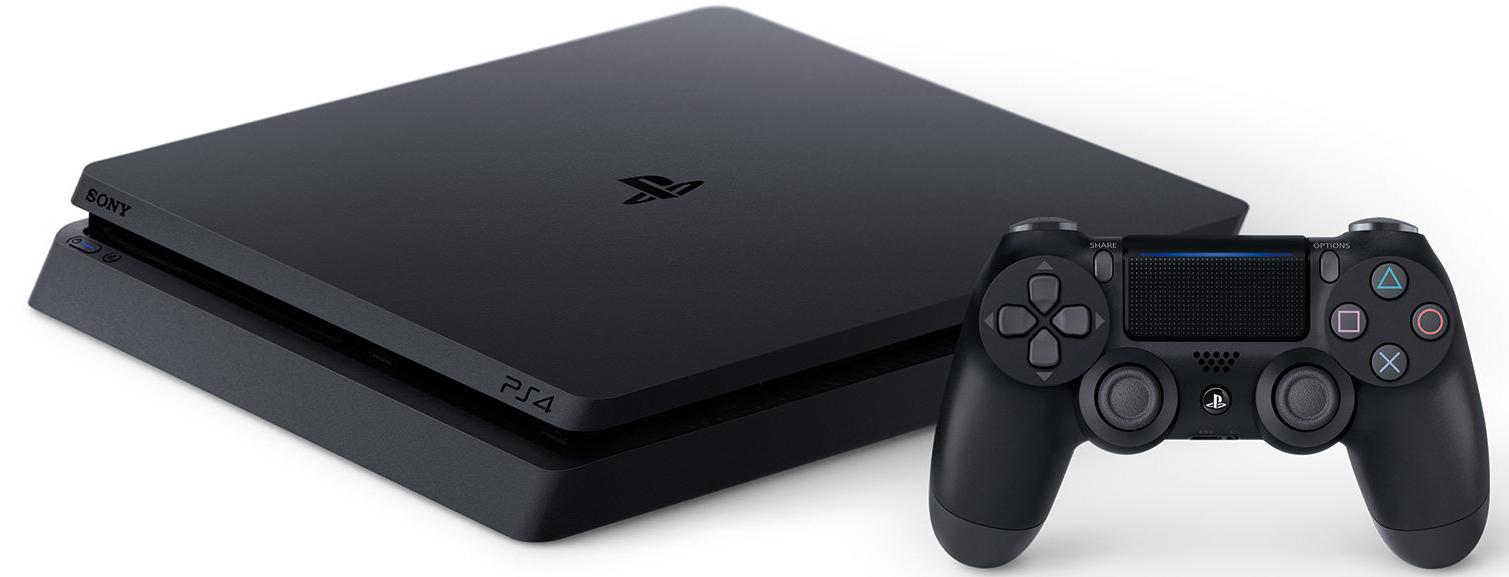
\includegraphics[width=0.5\textwidth]{ps4}
            \caption{Playstation 4 mit Controller}\label{fig:ps4}
        \end{figure}

        Gesteuert wird die Konsole in der Regel, durch einen Controller, welcher hauptsächlich für Spiele konzipiert wurde.
        Alternativ können auch diverse Bluetooth-Geräte oder eine Smartphone-App genutzt werden.

    \item[Raspberry Pi \cite{Whatisth47:online}]
        Der Raspberry Pi ist ein Einplatinencomputer \cite{Einplati37:online}, also ein Computer,
        bei welchem sich alle benötigten Komponenten auf einer einzigen Leiterplatte befinden.
        In diesem Projekt wird das Modell \textit{Raspberry Pi 3 Model B} verwendet.
        Hierzu zählen beim Raspberry Pi unter anderem die CPU, ein HDMI-Anschluss, mehrere USB-Buchsen sowie ein LAN-Anschluss.
        Betrieben wird er über ein Betriebssystem, welches auf einer Micro-SD installiert wird.

        \begin{figure}[h!]
            \centering
            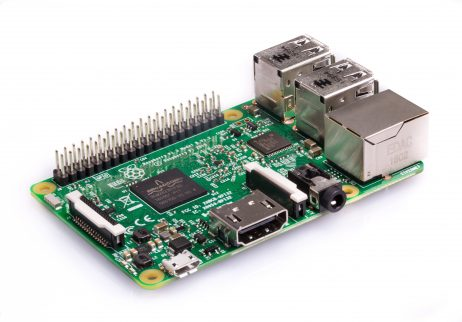
\includegraphics[width=0.5\textwidth]{pi}
            \caption{Raspberry Pi 3 Model B \cite{Raspberr2:online}}\label{fig:pi}
        \end{figure}

        Das offiziell unterstütze Betriebssystem ist \textit{Raspbian}, welches auf dem Linux-Betriebssystem \textit{Debian} basiert.
        Mit diesem Betriebssystem bietet der Raspberry Pi nahezu alle Möglichkeiten, welche auch ein klassischer Computer bietet.
        Eine Einschränkung ist jedoch, dass der Pi lediglich einen ARM-Prozessor besitzt.
        Programme, welche nur für x86- oder x64-Prozessoren entwickelt wurden, können somit nicht ausgeführt werden.

        Anstelle von \textit{Raspbian} können auch andere Betriebssysteme installiert werden,
        welche besser auf einen bestimmten Anwendungsfall zugeschnitten sind.

    \item[Home Assistant \cite{HomeAssi51:online}]
        Home Assistant ist eine open-source Plattform zur Heimautomatisierung.
        Basierend auf der Programmiersprache \textit{Python 3} ist sie gedacht,
        um auf einem Raspberry Pi ausgeführt zu werden.
        Mit \textit{Hassbian} wird ein Betriebssystem basierend auf \textit{Raspbian} angeboten,
        auf welchen Home Assistant bereits installiert und grundlegend konfiguriert ist.

        \begin{figure}[h!]
            \centering
            
\includegraphics[width=0.25\textwidth]{homeassistant}
            \caption{Logo Homeassistant}\label{fig:homeassistant}
        \end{figure}

        Die Plattform ermöglicht das Überwachen und Steuern verschiedener Geräte zu Heimautomatisierung.
        Für dieses Projekt wird sie so konfiguriert,
        dass sie den Status der Playstation 4 überwacht und das Ein- sowie Ausschalten ermöglicht.
        Details zu dieser Konfiguration finden sich in Kapitel \ref{sec:aufbau} \textit{\nameref{sec:aufbau}}.

    \item[Logitech Harmony \cite{HarmonyH15:online}]
        Logitech Harmony ist die Fernbedienungs-Sparte von Logitech.
        In diesem Projekt wird der Harmony Hub zusammen mit der zugehörigen Harmony Elite Fernbedienung verwendet,
        Durch den Harmony Hub könne zahlreiche Geräte über Infrarot, WLAN oder Bluetooth gesteuert werden.
        Die Fernbedienung selbst kommuniziert hierbei über Funk \cite{HowToPoi90:online} mit dem Hub.
        Der Hub gibt die Befehle dann an die entsprechenden Geräte weiter.
        Zusätzlich lässt sich der Hub über eine Smartphone-App ansteuern.

        \begin{figure}[h!]
            \centering
            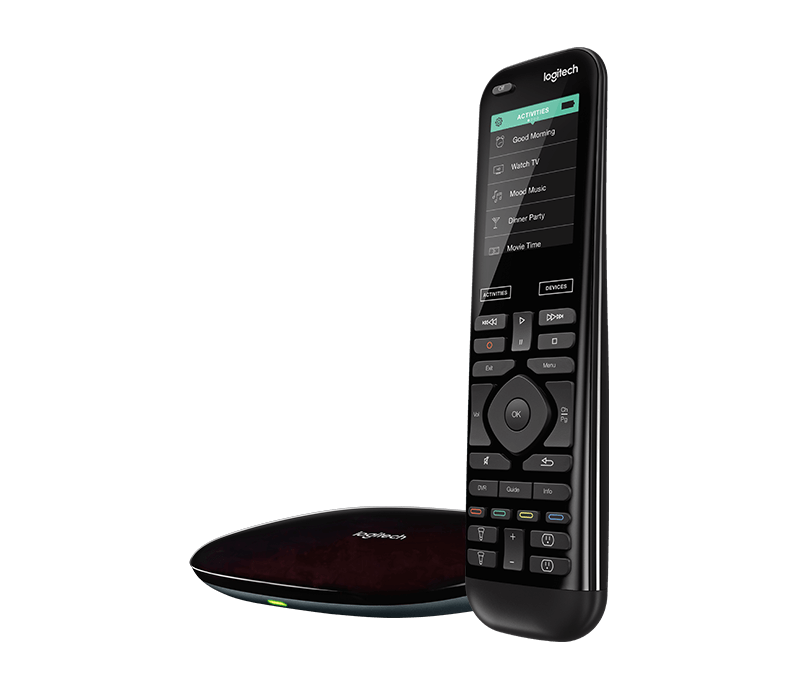
\includegraphics[width=0.5\textwidth]{harmony-elite}
            \caption{Hub, Fernbedienung und Smartphone mit App}\label{fig:harmony}
        \end{figure}

        Neben den verschiedenen Verbindungsmöglichkeiten ist ein großer Vorteil das Konfigurieren von \enquote{Aktionen}.
        Diese Stellen eine Sammlung von Befehlen an verschiedene Geräte dar.
        So kann beispielsweise über einen Tastendruck gleichzeitig Fernseher und Receiver eingeschaltet
        und (entsprechende Smart-Home-Geräte vorausgesetzt) das Licht gedimmt werden.
\end{description}
\newpage
\section{Aufbau und Konfiguration}\label{sec:aufbau}
In \autoref{fig:aufbau} wird grundlegend dargestellt,
wie die im vorigen Kapitel beschriebenen Komponenten miteinander verbunden sind.
Hierbei ist anzumerken, dass Verbindungen über (W)LAN indirekt über einen Router erstellt werden.
Zur Wahrung der Übersichtlichkeit zeigt die Abbildung
 lediglich die abstrakten Verbindungen auf Anwendungsebene.

\begin{figure}[ht!]
    \centering
    \resizebox{\textwidth}{!}{
        \input{assets/uml/Aufbau.latex}
    }
    \caption{Aufbau}
    \label{fig:aufbau}
\end{figure}

Im Folgenden werden die verschiedenen Konfigurationen der einzelnen Geräte vorgestellt.

\subsection{Harmony Hub}\label{sec:aufbau-hub}
Um den Harmony Hub als Fernbedienung für die Playstation 4 zu nutzen,
ist im Vorfeld das bei Bluetooth-Geräten übliche \enquote{Pairing} notwendig.

\newpage

\subsection{Raspberry Pi}\label{sec:aufbau-hassbian}

\paragraph{Steuern der \ac{ps4}}
Die Playstation lässt sich zwar per Bluetooth steuern,
kann auf diesem Weg allerdings nicht eingeschaltet werden.

Das Programm \textit{ps4-waker} hingegen erlaubt es die \ac{ps4} ein- sowie auszuschalten und sogar Anwendungen zu starten.

Das Einschalten geschieht über einen Befehl der Form \lstinline[language=bash]{ps4-waker -d 192.168.178.34  -c ~/.homeassistant/.ps4-wake.credentials.json}.
Durch \lstinline[language=bash]{-d} wird hierbei die IP-Adresse des Gerätes und
durch \lstinline[language=bash]{-c} die Datei,
welche die notwendigen Zugangsdaten enthält, angegeben.

Die Zugangsdaten werden zuvor durch folgendes Pairing-Verfahren ermittelt:
\begin{enumerate}
    \setlength\itemsep{-0.5em}
    \item \textit{ps4-waker} gibt sich beim ersten Start als Playstation 4 aus.
    \item Mit einem Smartphone wird versucht sich über die entsprechende App mit der \enquote{falschen} \ac{ps4} zu verbinden.
    \item \textit{ps4-waker} nutzt die so übertragenen Informationen, um sich gegenüber der \enquote{echten} \ac{ps4} als Smartphone-App auszugeben.
    \item Die so erhaltenen Zugangsdaten werden in einer JSON-Datei gespeichert.
\end{enumerate}

Durch Anhängen des Schlüsselworts \enquote{\lstinline[language=bash]{standby}} kann die
\ac{ps4} wieder ausgeschaltet werden.

Um \textit{ps4-waker} innerhalb von Home Assistant zu nutzen,
werden sogenannte \textit{Schalter} konfiguriert.
Unter anderem können diese Schalter genutzt werden, um Kommandozeilenbefehle (\ac{cli})
im darunterliegenden Betriebssystem auszuführen.

In \autoref{lst:ps4_switch} ist die Konfiguration des Schalters dargestellt,
welcher zum Ein- und Ausschalten der Playstation 4 dient.

\lstinputlisting[
    caption=Konfiguration des Schalters,
    label=lst:ps4_switch,
    language=yaml
]{ps4_switch.yaml}

Die erste Zeile gibt die eindeutige ID für den Schalter an.
Durch den \lstinline[language=yaml]{friendly_name} kann zusätzlich ein nutzerfreundlicher Name zur Anzeige auf Benutzeroberflächen angegeben werden.

Der aktuelle Zustand des Schalters wird mit \lstinline[language=yaml]{command_state}
und \lstinline[language=yaml]{value_template} ermittelt.
Der Kommandozeilenbefehl \lstinline[language=yaml]{command_state} wird regelmäßig ausgeführt.
Als Ergebnis liefert er die in \autoref{lst:ps4-waker_search} dargestellten Daten im JSON-Format.
In \lstinline[language=yaml]{value_template} wird auf dieses JSON über
\lstinline[language=yaml]{'value_json'} zugegriffen.
Genauer gesagt wird geprüft,
ob das Feld \lstinline[language=json]{"statusCode"} den Wert
\lstinline[language=json]{"200"} enthält.
Ist dies der Fall, so gilt der Schalter als eingeschaltet, andernfalls als ausgeschaltet.

\lstinputlisting[
    caption=Antwort von \textit{ps4-waker search}-Befehl (gekürzt),
    label=lst:ps4-waker_search,
    language=json
]{ps4-waker_search.json}

Je nach aktuellem Status des Schalters führt ein Betätigen dazu, dass der Kommandozeilenbefehl \lstinline[language=yaml]{command_on} zum Einschalten
oder der \lstinline[language=yaml]{command_off} zum Ausschalten ausgeführt wird.
Beides wird über die jeweiligen Befehle von \textit{ps4-waker} umgesetzt.

\paragraph{LAN-Schnittstelle}
Der Schalter kann ohne Weiteres nicht durch den Harmony Hub gesteuert werden,
da keine gemeinsame Schnittstelle vorhanden ist.

Diese Aufgabe übernimmt eine emulierte \textit{Hue Bridge}.
Eigentlich ist die \textit{Hue Bridge} zentraler Bestandteil des smarten Lampensystems der Marke Phillips \cite{HueBridg65:online}.
Im Home-Assistant wird die emulierte \textit{Hue Bridge} so konfiguriert,
dass sie den Schalter gegenüber dem Harmony Hub als Leuchte präsentiert.
Da im Harmony Hub das Kontrollieren von Leuchten einer \textit{Hue Bridge} möglich ist,
kann auf diesem Weg der Schalter ein- und ausgeschaltet werden.

\subsection{Netzadressen}\label{sec:aufbau-adressen}
Die folgende Tabelle zeigt die jeweiligen IP- und MAC-Adressen anhand welcher die
späteren Paketmitschnitte analysiert werden. \\

\begin{center}
    \begin{tabular}{l||c|c}
        Gerät           & IP-Adresse                &  MAC-Adresse          \\
        \hline
        \hline
        Harmony Hub     & \texttt{192.168.178.21}  &  \texttt{C8:DB:26:00:D0:E9}  \\
        \hline
        Raspberry Pi    & \texttt{192.168.178.45}  &  \texttt{B8:27:EB:9F:0E:FE}  \\
        \hline
        Playstation     & \texttt{192.168.178.34}  &  \texttt{80:EA:23:19:B6:5C}   \\
    \end{tabular}
\end{center}


\section{Ablauf}\label{sec:ablauf}
Zur Untersuchung der Kommunikation zwischen der Geräten wird der Verkehr auf den LAN-Schnittstellen in verschiedenen Szenarien betrachtet:

\begin{enumerate}
    \item Ein- und Ausschalten über \textit{Hassbian}
    \item Ein- und Ausschalten über \textit{Harmony Hub}
\end{enumerate}

Eine detaillierte Beschreibung der Szenarien folgt in Kapitel. \todo[inline]{Kapitel hinzufügen}


Alle in den Szenarien betrachteten Verbindungen sind LAN-Verbindungen und werden über den zentralen Router des lokalen Netzwerk transportiert.
Folglich ist dies auch eine nützliche Stelle um den anfallenden Verkehr mitzuschneiden.
In diesem Fall handelt es sich bei dem Router um eine \textit{FRITZ!Box 7560}\cite{FRITZBox29:online}.
Wie auch andere FRITZ!Boxen stellt diese unter der Adresse \url{http://fritz.box/html/capture.html} eine Oberfläche bereit,
um Datenpakete an verschiedenen Schnittstellen mitzuschneiden
und in einem für das bekannte Tool \textit{Wireshark} lesbaren Format herunterzuladen.

\begin{figure}[ht!]
    \centering
    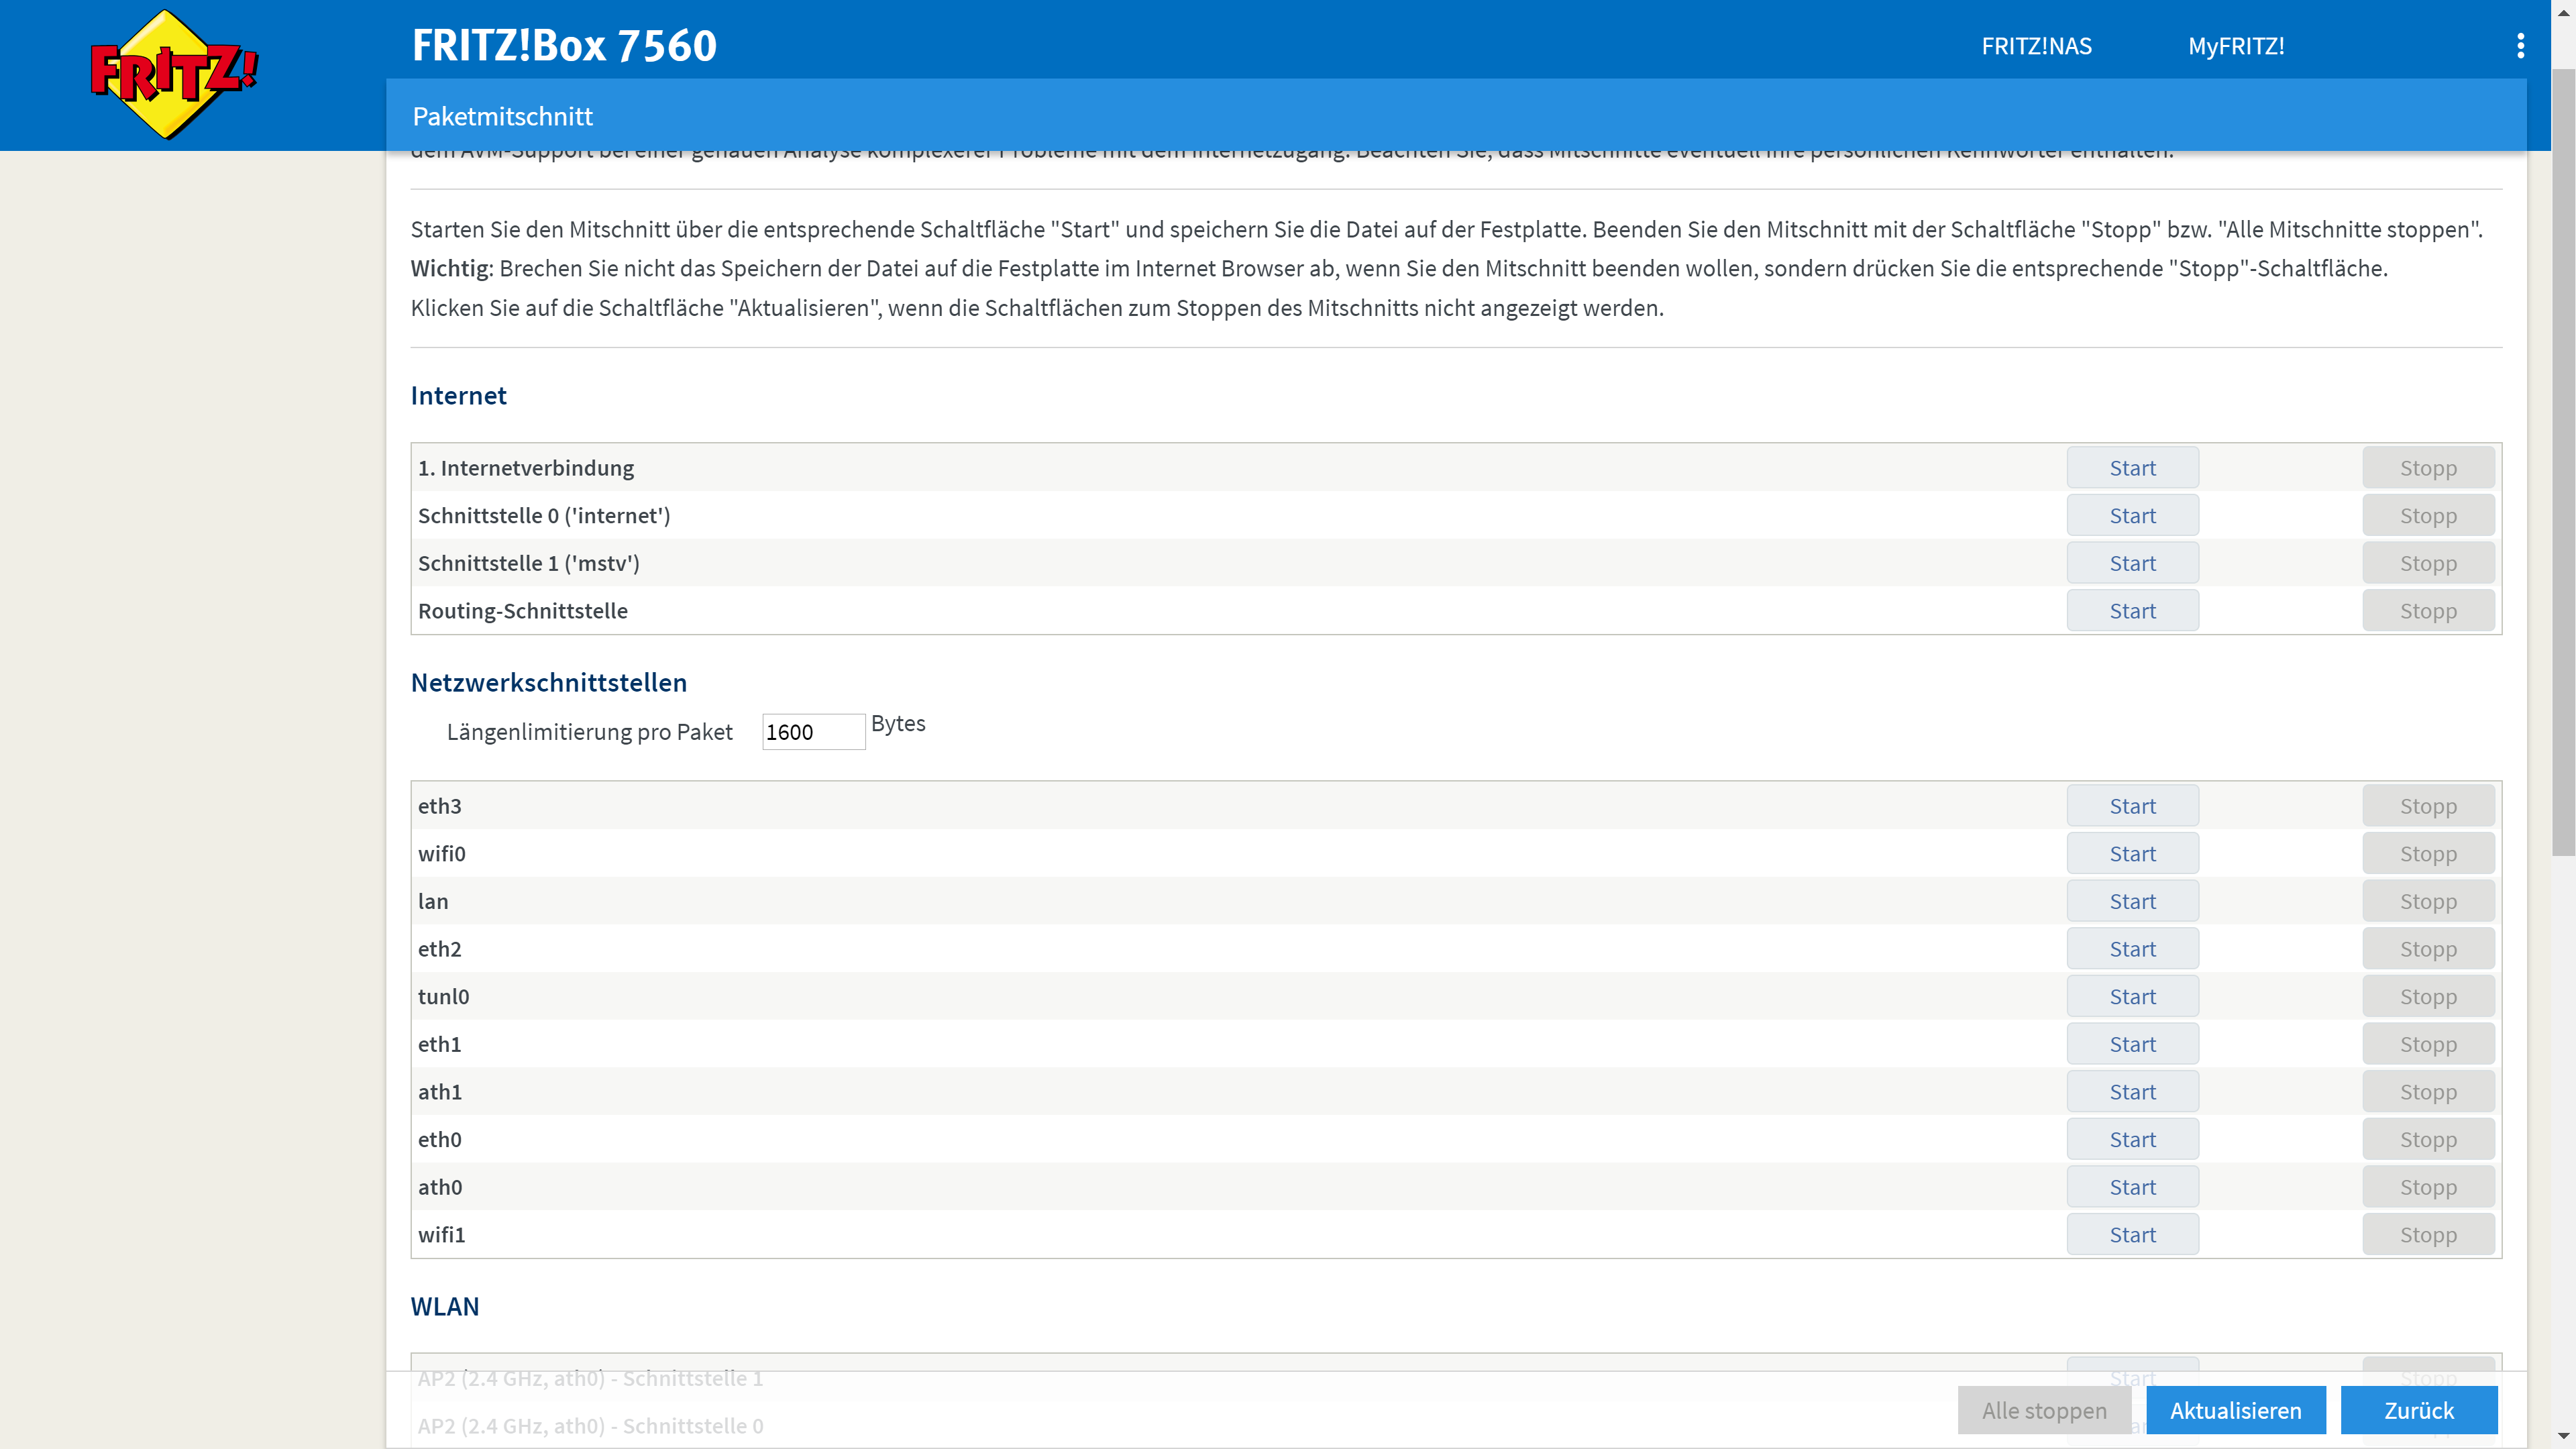
\includegraphics[width=\textwidth]{fribCapture}
    \caption{FRITZ!Box Weboberfläche für Paketmitschnitte}\label{fig:fribCapture}
\end{figure}

Diese Methode bringt zwei entscheidente Vorteile mit sich:
Zum Einen läufte der gesamte Verkehr durch den Router, da alle Geräte per (W)LAN an diesen angeschlossen sind.
Zum Anderen können dort die Pakete unkompliziert mitgeschnitten werden. Zugriff auf die zu betrachtenden Geräte
oder gar ein Umleiten des Verkehrs auf einen Computer, beispielsweise durch \textit{Spoofing}\cite{Maninthe12:online} sind nicht notwendig.

Jedoch hat diese Methode auch einen Nachteil:
Die Oberfläche für Paketmitschnitte ist nicht für den allgemeinen Nutzer,
sondern eigentlich zur Unterstützung des Supports bei kopmplexen Problemen bestimmt.
Daher wird die Seite auch nicht detailliert dokumentiert.
Lediglich eine kurze Anleitung wie solle Paketmitschnitte gestartet und gestoppt werden befindet sich im oberen Bereich der Seite.
Die in \autoref{fig:fribCapture} zu sehenden zahlreichen Schnittstellen werden nicht näher spezifiziert.

In \cite{fritzcap8:online} präsentiert Jeroen Wiert Pluimers die Ergebnisse einer Analyse der Schnittstellen.
Hier hervorzuheben ist die Schnittstelle \texttt{ath0}. Als WLAN-Schnittstelle scheint sie gut für dieses Projekt geeignet zu sein.

Ein rudimentärer praktischer Vergleich mit den Schnittstellen \texttt{lan} und \textit{Routing-Schnittstelle} zeigt,
dass in dem Mitschnitt von \texttt{ath0} alle Pakete der zu betrachtenden Komponenten enthalten sind.

Der Mitschnitt von \texttt{lan} enthält zwar auch alle Pakete der zu betrachtenden Komponenten.
Enthält jedoch auch viele andere Pakete was zu einem erhöhten Overhead führt.

Der Mitschnitt der \textit{Routing-Schnittstelle} enthält lediglich Pakete welche vom Router an das Internet gesendet oder aus diesem Empfangenw werden.
Diese Schnittstelle ist daher für den lokalen Verkehr ungeeignet.\\

Das Erfassen der Pakete für eines der Szenarion folgt folgendem Muster:
\begin{enumerate}
    \setlength\itemsep{-0.5em}
    \item Starten des Paketmittschnitts auf \texttt{ath0}
    \item Durchführen des Szenarios
    \item Beeenden des Paketmittschnitts
    \item Öffnen des Mitschnitts mit \textit{Wireshark} und filtern der relevanten Pakete
    \item Speichern des gefilterten Mitschnitts zur späteren Analyse
\end{enumerate}
\newpage
\section{Durchführung}\label{sec:durchfuehrung}
In diesem Kapitel werden die Szenarien im Detail beschrieben,
sowie deren Paketmittschnitte analysiert.
Die Analyse beschränkt sich hierbei auf Nachrichten der Geräte untereinander
und auf mit dem Szenario zusammenhängende Pakete an andere Geräte/Server im Internet.

\subsection{Jeweils eine Minute ohne Aktionen bei ein- und ausgeschalteter Konsole}\label{sec:durchfuehrung-aus}
Ziel dieses Szenarios ist es die Kommunikation zu ermitteln,
welche zwischen den Geräten stattfindet,
ohne dass durch den Benutzer ein Befehl erteilt wurde.
Es zeigt sich, dass die Geräte auch im Ruhezustand rege miteinander Informationen austauschen.

\paragraph{Home Assistant und Playstation 4}
Der Home Assistant wurde so konfiguriert,
dass er regelmäßig den Status der \ac{ps4} überprüft.
Dies geschieht über ein UDP-Paket,
welches an Port \texttt{987} der Broadcast-Adresse \texttt{255.255.255.255} gesendet wird.
Über das Senden an die Broadcast-Adresse wird erreicht,
dass der Router das Paket an alle lokalen Geräte verteilt.
\texttt{987} wiederum ist der Port, über welchen die Spielekonsole UDP-Pakete annimmt.

Der Inhalt des Pakets (siehe \autoref{lst:ps4-wakeup_search}) besteht aus dem Kommando \texttt{SRCH},
der HTTP-Version und einer \texttt{device-discovery-protocol-version}.
Vermutlich steht das Kürzel \texttt{SRCH} für \enquote{Search}.
Mit diesem Paket werden keine Aktionen ausgeführt,
sondern nur Systeminformationen angefordert.

\lstinputlisting[
    caption=Daten eines SRCH-Paketes,
    label=lst:ps4-wakeup_search
]{ps4_search.udp}

\newpage

Auf dieses Paket antwortet die \ac{ps4} ebenfalls mit einem UDP-Paket,
welches verschiedenen Geräteinformationen enthält.

Vergleicht man die Antworten der eingeschalteten (\autoref{lst:ps4-wakeup_search_respOn})
und ausgeschalteten (\autoref{lst:ps4-wakeup_search_respOff}) \ac{ps4} miteinander,
so ist festzustellen,
dass sich die jeweiligen Antworten lediglich im Statuscode der ersten Zeile unterscheiden.
\texttt{200 Ok} gibt an, dass die Playstation 4 eingeschaltet und \texttt{620 Server Standby},
dass die ausgeschaltet (bzw. im Standby-Modus) ist.

\lstinputlisting[
    caption=Antwort auf SRCH-Paket (Eingeschaltet),
    label=lst:ps4-wakeup_search_respOn
]{ps4_search_respOn.udp}

\lstinputlisting[
    caption=Antwort auf SRCH-Paket (Ausgeschaltet),
    label=lst:ps4-wakeup_search_respOff
]{ps4_search_respOff.udp}

\newpage
\paragraph{Home Assistant und Harmony Hub}
Um ebenfalls regelmäßig den aktuellen Status der Spielekonsole zu erfahren,
erfragt der Harmony Hub diese Information beim Home Assistant über die emulierte \textit{Hue Bridge}.
Dies geschieht in Form eines HTTP-GET-Requests,
welcher über eine für diesen Zweck errichte TCP-Verbindung erfolgt.
Der Request erfolgt an die URL \nolinkurl{192.168.178.45:8300/api/12345678901234567890/lights}.

Über den Port \texttt{8300} wird die emulierte \textit{Hue Bridge} erreicht,
welche über den angegebenen Pfad Informationen über alle eingerichteten \enquote{Leuchten}
(darunter auch der Schalter zur Kontrolle der \ac{ps4}) bereitstellt.

Als Antwort liefert Home Assistant mehrere Objekte im JSON-Format.
Der Teil der Antwort welcher den Schalter,
ist in \autoref{lst:ps4_get} dargestellt.
Hervorzuheben sind hier folgende Felder:
\lstinline[language=json]{"name"} enthält den nutzerfreundlichen Namen,
welcher in der Konfiguration angegeben wurde.
\lstinline[language=json]{"uniqueid"} enthält die
in der Konfiguration gesetzte ID mit dem zusätzlichen Präfix \lstinline[language=json]{"switch"}.
Das Feld \lstinline[language=json]{"on"} gibt an, ob die Leuchte (und damit die Spielekonsole) gerade eingeschaltet ist.
In diesem Fall ist sie ausgeschaltet, weshalb dieser Wert \lstinline[language=json]{false} ist.

\lstinputlisting[
    caption=Nutzdaten GET-Response (gekürzt),
    label=lst:ps4_get,
    language=json
]{ps4_get.json}

\newpage

\subsection{Ein- und Ausschalten über Home Assistant}\label{sec:durchfuehrung-hassbian}
\hyphenation{Web-ober-fläche}
Der Home Assistant bietet zur Steuerung der konfigurierten Geräte eine Weboberfläche.
In \autoref{fig:hass-ui} ist der Schalter hervorgehoben, welcher für das Ein- und Ausschalten der Playstation 4 genutzt wird.

\begin{figure}[h!]
    \centering
    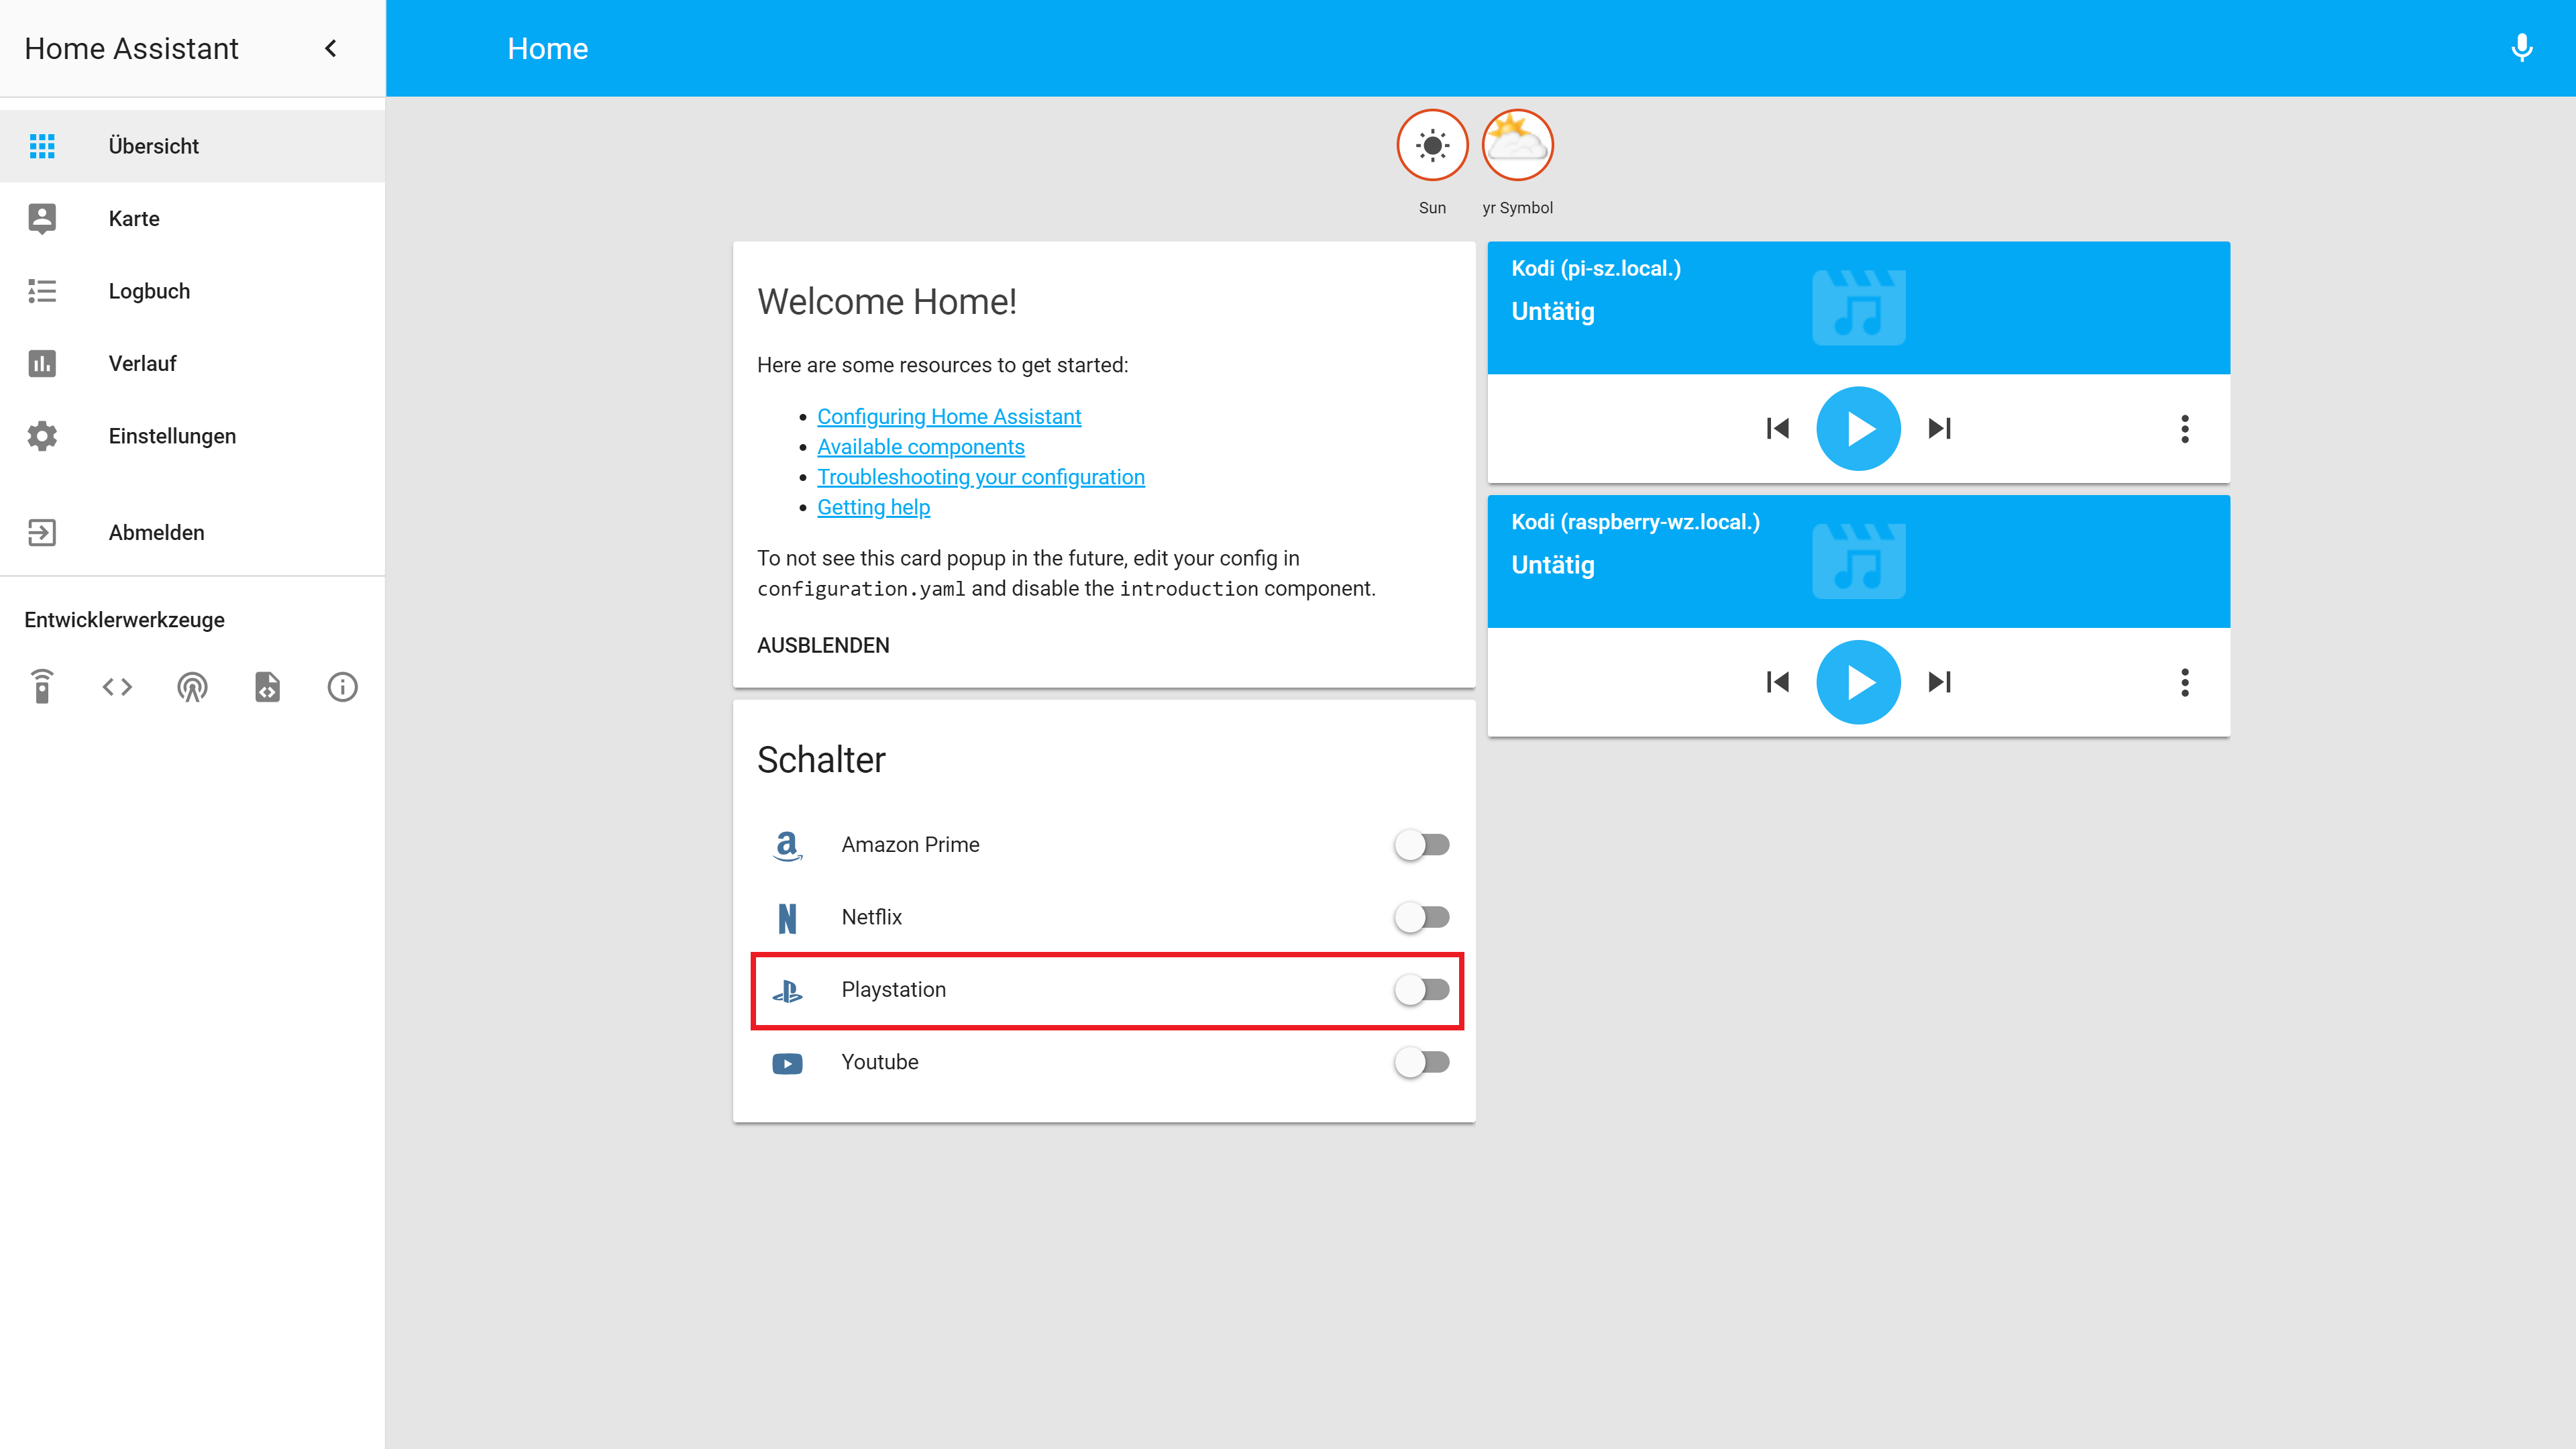
\includegraphics[width=\textwidth]{hass_ui}
    \caption{Weboberfläche des Home Assistant}\label{fig:hass-ui}
\end{figure}

Sowohl beim Ein- als auch beim Ausschalten werden zusätzlich zu dem bereits bekannten \texttt{SRCH}-Paket
zwei weitere Arten von UDP-Paketen gesendet.
Das eine enthält den Befehl \texttt{WAKEUP} (\autoref{lst:ps4-wakeup}),
das andere den Befehl \texttt{LAUNCH} (\autoref{lst:ps4-launch}).

\lstinputlisting[
    caption=Daten eines WAKEUP-Paketes,
    label=lst:ps4-wakeup
]{ps4_wakeup.udp}


Das Feld \texttt{user-credential} (in den Listings gekürzt) ist hierbei immer gleich.
Der darin enthaltene Wert wurde beim initialen Verbindungsaufbau automatisch ermittelt.
Es werden zwei \texttt{WAKEUP}-Pakete und ein \texttt{LAUNCH}-Paket gesendet,
um zu prüfen, ob die \ac{ps4} bereit ist eine Verbindung anzunehmen.

\lstinputlisting[
    caption=Daten eines LAUNCH-Paketes,
    label=lst:ps4-launch
]{ps4_launch.udp}

Der eigentliche Befehl wird in einer, auf die UDP-Pakete folgenden, TCP-Verbindung ausgeführt.
Zwar ist diese Verbindung nicht mit TLS verschlüsselt,
die Daten können dennoch nicht ausgelesen werden.

Der Grund hierfür ist im Quellcode des \textit{ps4-waker} ersichtlich \cite{ps4waker31:online}\cite{ps4waker93:online}:
Die Daten werden dort vor dem Senden (und damit auf Anwendungsebene) verschlüsselt.
Ein weiterer Blick in den Quellcode zeigt den Aufbau der TCP-Pakete.
Der Paket-Typ (auf Anwendungsebene) wird durch eine Ganzzahl angegeben.
Zusätzlich werden je nach Anwendungsfall ASCII Zeichen oder Ganzzahlen übertragen,
um die gewünschten Befehle auszuführen.
Das Paket eines Standby-Befehls wird beispielsweise wie in \autoref{lst:ps4-standby} erstellt und gesendet (aus \cite{ps4waker31:online}).

\lstinputlisting[
    caption=Erstellen und Senden eines Standby-Befehls,
    label=lst:ps4-standby,
    firstnumber=273
]{ps4_standby.js}

Durch diese Funktionsaufrufe wird ein TCP-Paket der Länge 8 Bytes erstellt,
mit der Zahl 26 gefüllt,
verschlüsselt und gesendet.

\newpage

\subsection{Ein- und Ausschalten über \textit{Harmony Hub}}\label{sec:durchfuehrung-harmony}
Im Harmony Hub ist zur Nutzung der Playstation 4 eine Aktion namens \enquote{Spielen} konfiguriert.
Zusätzlich zur Spielekonsole wird in dieser Aktion auch der Fernseher ein- bzw. ausgeschaltet.

Zum Einschalten wird der durch den Home Assistant bereitgestellte Schalter genutzt.
Dieser wird über die emulierte \textit{Hue Bridge} durch den Harmony Hub aktiviert.

Ist die \ac{ps4} eingeschaltet, so kann der Hub eine Bluetooth-Verbindung aufbauen.
Daher ist es zum Ausschalten nicht nötig den Home Assistant zu nutzen.
Der Hub schaltet die Konsole direkt über die Bluetooth-Verbindung aus,
sobald die Aktion \enquote{Spielen} beendet wird.

\subsubsection{Einschalten}
Der Paketmitschnitt enthält mehrere TCP-Verbindungen.
An der Kommunikation sind der Harmony Hub, der \textit{Home Assistant} und die \ac{ps4} beteiligt.
Zusätzlich frägt der Harmony Hub per DNS die IP-Adresse von \nolinkurl{home.myharmony.com} an.
Als Antwort wird auf den Server mit der URL \nolinkurl{home-myharmony.us-east-1.elasticbeanstalk.com} verwiesen.
Die TCP-Verbindung zwischen Harmony Hub und Webserver ist durch TLS verschlüsselt.

Der \textit{Home Assistant} und die \ac{ps4} kommunizieren, wie bereits im vorigen Abschnitt untersucht, mittels TCP und UDP.
Der Harmony Hub kommuniziert mit \textit{Home Assistant} über HTTP.

Der Ablauf der Kommunikation wird in \autoref{fig:ps-ein-harmony} vereinfacht dargestellt.
Bei HTTP-Verbindungen wird lediglich das HTTP-Paket gezeigt,
der TCP-Rahmen mit Verbindungsaufbau und -abbau wird nicht abgebildet.
Außerdem fehlen in der Abbildung die UDP-Pakete,
welche vom \textit{Home Assistant} genutzt werden,
um den Status der \ac{ps4} zu erfragen.

\begin{figure}
    \centering
    \resizebox{\textwidth}{!}{
        \input{assets/uml/ps-ein-harmony.latex}
    }
    \caption{Kommunikation beim Einschalten}
    \label{fig:ps-ein-harmony}
\end{figure}

\newpage



\paragraph{Harmony Hub und Webserver}
Die Verbindungen sind verschlüsselt.
Daher können zum genauen Inhalt und Zweck keine Aussagen getroffen werden.
Vermutlich dienen sie dazu, Informationen über die gestartete Aktion zu übergeben.

Bei genauerer Betrachtung eines Paketes, welches vom Harmony Hub an den Webserver gesendet wird,
sind verschiedene Besonderheiten zu erkennen:

\begin{figure}[h!]
    \centering
    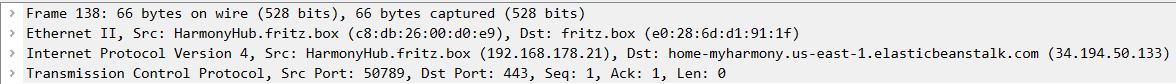
\includegraphics[width=\textwidth]{internet-paket}
    \caption{Paket von Harmony Hub an Webserver}\label{fig:internet-paket}
\end{figure}


\autoref{fig:internet-paket} zeigt die verschiedenen Protokoll-Header, welche ineinander verschachtelt sind.
Die oberste Zeile (\textit{Frame}) steht für das gesamte Paket.

In der zweiten Zeile steht die äußerste Paket-Schicht \textit{Ethernet II}.
Deren Quelladresse ist die MAC-Adresse des Harmony Hub.
Als Zieladresse ist jedoch nicht die MAC-Adresse des Webservers,
sondern die der FRITZ!Box angegeben.
Dies liegt daran, dass Ethernet lediglich zur Kommunikation im lokalen Netz verwendet wird.
Das Paket wird per Ethernet an die FRITZ!Box gesendet.
Dort wird die \enquote{Ethernet-Nutzlast} (das IP-Paket inklusive TCP; Zeile 3) entpackt und über \textit{IPv4} an das eigentliche Ziel weitergeleitet.
Dessen Adresse ist als Zieladresse im IP-Header angegeben.

Da die Verbindung verschlüsselt ist, lassen sich aus den übertragenen Daten keine Informationen gewinnen.
Der Zielport des TCP-Headers in der letzten Zeile liefert jedoch einen Hinweis auf die Methode der Übertragung.
Der Port \textit{443} wird standardmäßig für \textit{HTTPS}-Verbindungen genutzt.
Daraus und aus der Tatsache, dass die Verbindung mittels TLS verschlüsselt ist,
lässt sich mit hoher Wahrscheinlichkeit schließen, dass tatsächlich \textit{HTTPS} genutzt wird.

\paragraph{Home Assistant und Playstation 4}
Zwischen diesen Geräten läuft die Kommunikation nach dem gleichen Schema ab,
wie es bereits im vorigen Abschnitt betrachtet wurde.

\paragraph{Home Assistant und Harmony Hub}
Auch während des Einschaltens werden HTTP-GET-Requests (siehe Kapitel \ref{sec:durchfuehrung-aus}) genutzt,
um vom Harmony Hub aus den Status der \ac{ps4} zu erfragen.

Zusätzlich wird ein HTTP-PUT-Request gesendet, wodurch der Befehl das Gerät einzuschalten übermittelt wird.
Dieser Request wird an die Adresse \nolinkurl{http://192.168.178.45:8300/api/12345678901234567890/lights/1/state} gesendet.

Die angegebene IP-Adresse ist die des Raspberry PI, welcher an Port 8300 Befehle an die emulierte \textit{Hue Bridge} des \textit{Home Assistant} entgegennimmt.
\texttt{/api/\\12345678901234567890/lights/1} wählt das zu kontrollierende Gerät aus.
Wie in Kapitel \ref{sec:aufbau-hassbian} beschrieben, werden die Geräte nach außen hin als Lichter (engl. Lights) präsentiert.
Als Nutzdaten enthält das Paket die in \autoref{lst:ps4_on-request} gezeigten Daten im JSON-Format.

\lstinputlisting[
    caption=Nutzdaten PUT-Request,
    label=lst:ps4_on-request,
    language=json
]{ps4_on-request.json}

Für diesen Anwendungsfall ist einzig der Wert \lstinline[language=json]{"on": true} von Relevanz.
Mit dem Wert \lstinline[language=json]{"x,y"} könnte bei echten Lampen die Farbe
und mit dem Wert \lstinline[language=json]{"bri"} die Helligkeit gesteuert werden \cite{Coreconc26:online}.


Die Antwort auf den PUT-Request enthält ebenfalls Daten im JSON-Format,
um den Erfolg des Befehls mitzuteilen (siehe \autoref{lst:ps4_on-response}).
\lstinputlisting[
    caption=Nutzdaten PUT-Request,
    label=lst:ps4_on-response,
    language=json
]{ps4_on-response.json}

\newpage
\subsubsection{Ausschalten}
Da zum Ausschalten der \ac{ps4} der \textit{Home Assistant} nicht genutzt wird,
fällt die Netzwerkkommunikation hier deutlich sparsamer aus.

Wieder kommuniziert der Harmony Hub verschlüsselt mit \nolinkurl{home.myharmony.com}.
Außerdem wird der Status der Konsole vom Harmony Hub beim \textit{Home Assistant} über die bereits bekannten GET-Requests erfragt.
Der \textit{Home Assistant} erhält den Status der Konsole wiederum durch die SRCH-Pakete.

\begin{figure}[ht!]
    \centering
    \resizebox{\textwidth}{!}{
        \input{assets/uml/ps-aus-harmony.latex}
    }
    \caption{Kommunikation beim Ausschalten}
    \label{fig:ps-aus-harmony}
\end{figure}

In \autoref{fig:ps-aus-harmony} ist der Ablauf beim Ausschalten dargestellt.
Im Gegensatz zum vorigen Ablaufdiagramm sind hier die SRCH-Pakete abgebildet.
Außerdem ist zu den Antworten auf die Statusanfrage notiert,
ob die \ac{ps4} zu diesem Zeitpunkt ein- oder ausgeschaltet ist.

Aus dem Ablauf ist zu erkennen,
dass die Konsole zwischen dem zweiten GET- und dem zweiten SRCH-Paket ausgeschaltet wurde.
Da dies über einen anderen Kanal (Bluetooth) geschieht,
finden sich im Paketmittschnitt zum Ausschalten selbst keine Nachrichten.
\newpage

\section{Fazit}\label{sec:fazit}

Zwischen vielen Geräten wird zur Kommunikation der Standard HTTP,
bzw. bei der Kommunikation nach Außen sogar HTTPS verwendet.

Erfreulicherweiße ist die Kommunikation mit dem Webserver im Internet damit durch TLS geschützt.

Die interne Kokmmunikation mit der emulierten \textit{Hue Brige} hingegen ist nicht geschützt.
Weder Integrität noch Vertraulichkeit sind damit gesichert.
Somit kann ein Angreifer, der sich im internen Netzwerk befindet,
die gesendeten Pakete passiv mitlesen.
Dadurch erfährt er,
welche Geräte im Netzwerk über den \textit{Home Assistant} und die emulierte \textit{Hue Brige} gesteuert werden.

Weitaus schlimmer ist jedoch, dass er die GET- und POST-Requests auch selbst stellen kann.
Zum einen muss er dann nicht (ggf. aufwändig) das Netzwerk belauschen
und zum anderen kann er auf diesem Weg auch Geräte selbst steuern.

Für Privatanwender ist dies eine potentielle Bedrohung,
Allerdings ist davon auszugehen,
dass ein Angreifer im internen Netz aufgrund der überschaubaren Größe eher unwahrscheinlich ist.
Außerdem hält sich in diesem Beispiel der Schaden in Grenzen, da nur Unterhaltungsgeräte ein- bzw. ausgeschaltet werden.
Würde man auf gleiche Art und Weise ein Türschloss oder ähnliches kontrollieren erhöht das jedoch durch einen
möglichen Einbruch den potentiellen Schaden.

Im Gegensatz zu den anderen Übertragungen wird
in der TCP-Verbindung zwischen \textit{Home Assistant} und Playstation 4 kein allgemein bekannter Standard verwendet.
Die Verbindung ist zwar nicht über TLS, dafür aber auf Anwendungsebene verschlüsselt.
Hierdurch ist die Vertraulichkeit der Verbindung gesichert.
Zusätzlich werden jedoch ungesichert Pakete mittels UDP übertragen.

Zusammenfassend ist anzumerken,
dass ein großer Teil der Kommunikation über bekannte Standards bewältigt wird.
Zzumindest die Verbindungen, welche über das öffentliche Netz übertragen werden, sind gesichert.
Über die unverschlüsselten lokalen Verbindungen kann im Privatgebrauch in einem sicheren Netz hinweggesehen werden.
Sollte jedoch auch hier eine gesicherte Übertragung erforderlich sein,
so ist von dem hier gezeigten Aufbau abzuraten.

%\printacronyms{}
\newpage
\printbibliography{}
\end{document}